\subsubsection*{Cost Category 22.01.03: Compression Lasers}


%C_22_1_3 = 750*20/1.5; 



\begin{figure}
    \centering
    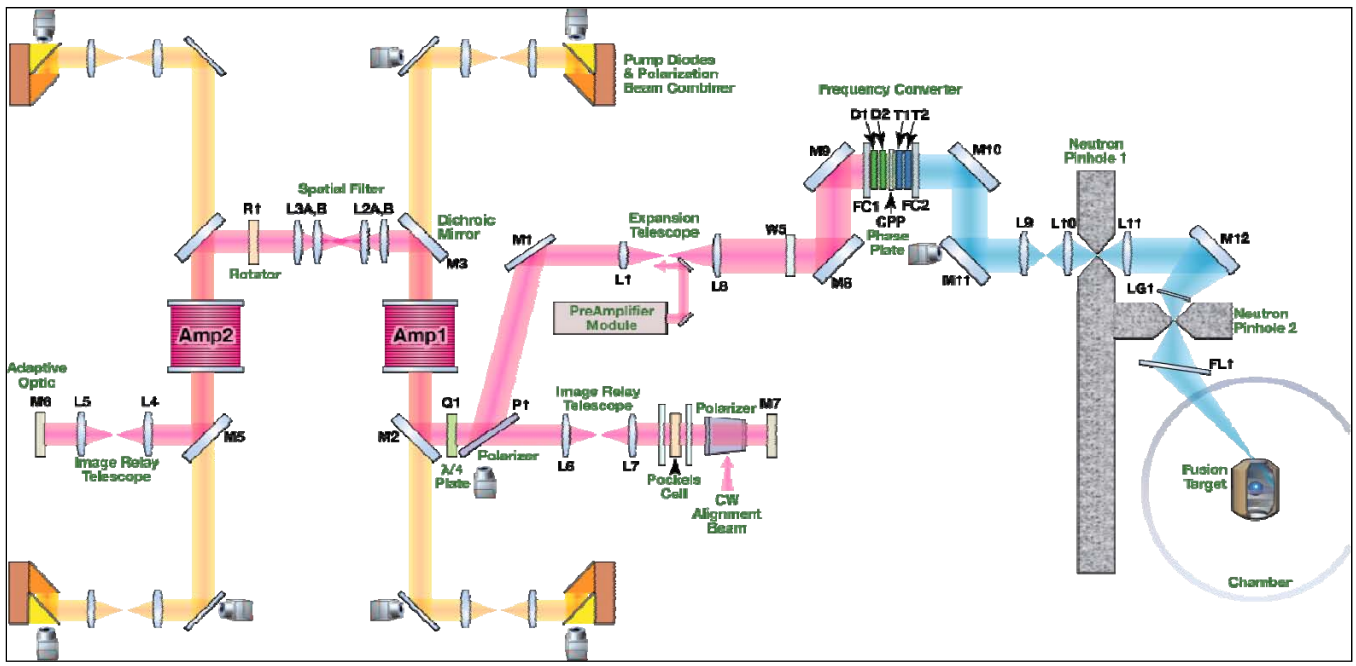
\includegraphics[width=0.9\linewidth]{Figures/Bayrmanian2011.png}
    \caption{LIFE laser architecture \cite{Bayramian2011}.}
    \label{fig:bayramian}
\end{figure}

%C_22_1_3 = 750*20/15; 


The Laser Inertial Fusion Energy (LIFE) concept, like other laser fusion systems, would also consist of various subsystems within its laser  
 system (see e.g. Fig.  \ref{fig:bayramian}). Although specific details can vary based on the design and technology used, here are some potential subsystems you might find within  the laser subsystem of a LIFE fusion system:    
   \begin{itemize} 
   \item Cost Category 22.01.03.01 Front End. This initial stage of the laser system is critical for generating the initial laser pulse. It sets the stage for subsequent amplification and conditioning, establishing the baseline characteristics of the laser pulse.
   \item Cost Category 22.01.03.02 Laser Amplification Subsystem. This subsystem involves multiple amplification stages that increase the energy of the laser pulse. Different types of amplifiers, such as solid-state or gas-based amplifiers, can be used.   
   \item Cost Category 22.01.03.03 Beam Transport Subsystem. This subsystem handles the precise transport of the laser beam from amplifiers to the target chamber. It includes optical components and beam-steering mechanisms.   
   \item Cost Category 22.01.03.04 Power conditioning system. Manages the electrical power needed for the laser system and ensures stable and reliable operation.
   \item Cost Category 22.01.03.05 Alignment and laser diagnostics.  Alignment and Calibration Subsystem: Maintains precise alignment of laser components to ensure accurate energy delivery to the target.
   \item Cost Category 22.01.03.06 Space frame. The space frame provides the structural support for the laser system. It ensures the physical stability and alignment of the various components, an aspect crucial for maintaining overall system integrity.
   \item Cost Category 22.01.03.07 Laser auxiliary systems. These systems encompass additional support mechanisms and technologies that assist in the operation and maintenance of the laser system, contributing to its overall functionality.
   \item Cost Category 22.01.03.08 Optics. The optics subsystem includes all the optical components involved in the laser system, such as lenses, mirrors, and diffraction gratings. They play a vital role in shaping, focusing, and directing the laser beam accurately towards its target.

   \end{itemize}   
   

\begin{table}[h!]
\centering
\resizebox{1\linewidth}{!}{%
\begin{tabular}{lcccc}
\hline
\textbf{Item} & \textbf{Procurement} & \textbf{Design} & \textbf{Assembly} & \textbf{Total} \\
\hline
22.1.3. Laser & 2036.9 & 140.4 & 382.1 & 1115.3 \\
\hspace{5mm}22.1.3.1 Front End & 172.1 & 20.9 & 36.7 & 100.1 \\
\hspace{5mm}22.1.3.2 Main Amp System & 460.6 & 25.5 & 76.2 & 245.0 \\
\hspace{10mm}22.1.3.2.1 Main Amp & 195.8 & 11.5 & 23.4 & 100.5 \\
\hspace{15mm}22.1.3.2.1.1 Flashlamp Assemblies & 49.3 & 0.0 & 0.0 & 21.5 \\
\hspace{15mm}22.1.3.2.1.3, 3.2.1.5-7 (amp mech) & 146.6 & 11.5 & 23.4 & 79.1 \\
\hspace{10mm}22.1.3.2.2 Spatial filters & 62.9 & 1.4 & 13.8 & 34.0 \\
\hspace{10mm}22.1.3.2.3 Mirror Mounts & 22.9 & 0.2 & 2.3 & 11.1 \\
\hspace{10mm}22.1.3.2.4 Polarizer assembly & 11.9 & 1.6 & 6.2 & 8.6 \\
\hspace{10mm}22.1.3.2.5 Pockels' Cell Assembly & 120.7 & 10.8 & 25.5 & 68.4 \\
\hspace{10mm}22.1.3.2.6 Boost Amp & 41.1 & 0.0 & 5.0 & 20.1 \\
\hspace{15mm}22.1.3.2.6.1 Flashlamp Assemblies & 10.6 & 0.0 & 0.0 & 4.6 \\
\hspace{15mm}22.1.3.2.6.3, 3.2.6.5-7 (amp mech) & 30.5 & 0.0 & 5.0 & 15.5 \\
\hspace{10mm}22.1.3.2.7 Interstage Hdw & 5.5 & 0.0 & 0.2 & 2.5 \\
\hspace{5mm}22.1.3.3 Beam Xport system & 130.6 & 6.4 & 21.8 & 69.2 \\
\hspace{10mm}22.1.3.3.1 Spatial filters & 71.4 & 5.3 & 0.0 & 33.4 \\
\hspace{10mm}22.1.3.3.2 Mirror Assembly & 19.3 & 0.2 & 16.5 & 15.7 \\
\hspace{10mm}22.1.3.3.3 Final Optics system & 28.7 & 0.7 & 2.1 & 13.7 \\
\hspace{10mm}22.1.3.3.4 Beam Tube system & 11.2 & 0.2 & 3.0 & 6.3 \\
\hspace{10mm}22.1.3.3.5 Interstage Hdw & 0.0 & 0.0 & 0.2 & 0.1 \\
\hspace{5mm}22.1.3.4 Power cond system & 226.5 & 0.0 & 0.0 & 98.7 \\
\hspace{5mm}22.1.3.5 Align and Laser diag & 163.9 & 36.3 & 112.0 & 136.0 \\
\hspace{5mm}22.1.3.6 Space frame & 51.6 & 8.3 & 0.0 & 26.1 \\
\hspace{5mm}22.1.3.7 Laser aux systems & 3.4 & 0.0 & 9.2 & 5.5 \\
\hspace{5mm}22.1.3.8 Optics & 0.0 & 0.0 & 0.0 & 0.0 \\
\hline
\end{tabular}}
\caption{NIF Costs Breakdown}
\label{tab:nif_costs}
\end{table}

 However, laser costs are forecast to come down, due mostly to mass production and automation of the manufacturing processes and  
 quality control in manufacturing using more advanced technologies.   
 This is just the usual learning curve - cost comes down at a rate that is proportional to the volume of production.  \\ 

 We have calibrated a learning curve to data from Leonardo (see accompanying document titled A Note on Learning Curve Credits for Laser Costs. 
 We apply the learning curve credits not only to the diodes, which constitute 20 \% of the laser cost, but also to the  
 optics and other laser components which with mass production and process automation will also follow a learning curve, so  
 by the 10th year, a factor of 10 reduction in cost should be anticipated.  We therefore state here the total cost of 20MJ  
 to be 1115 M \$.  This cost saving should occur within the first few years of production entailing multiple power plants. \\

Cost category 22.01.03: compression laser costs at  \$750/J for a 1.5MJ laser we get \$ 1115 M.


The cost bases for the NIF laser systems are available 
as an appendix for their 1993 design specification (see sheet ``NIF designs''). They presented four different designs, with varying pulse energy, wallplug efficiency etc. By plotting the cost of each subsystem for each design against the pulse energy, a first approximation of the relationship  can be determined and extrapolated (see sheet ''systems extrapolation'')

It turns out that from this sample, almost all systems can be simply linearly scaled with increasing energy, although more work  needs to be done here to better determine the extrapolation relationships.  Following this, and updating the costs according to inflation, a simple scaling of each subsystem to a specific energy requirement is found.

Also, when costing for NOAK, only the construction, and not pilot costs need to be considered. This approach has not yet, however, considered the economies of scale associated with a greatly increased batch 
number of e.g. laser beamlets.

The effect of this ''learning curve'' is dependent on the cost or time reduction between the first and average units (see ''learning curve'') for details). This treatment has been applied for both a 5x and 10x cost/time 
reduction following between the first and average components produced.

Laser costs are forecast to come down, due mostly to mass production and automation of the manufacturing processes and quality control in manufacturing using more advanced technologies. This is just the usual learning curve - cost comes down at a rate that is proportional to the volume of production. 

We have calibrated a learning curve to data from Leonardo (see accompanying document titled A Note on Learning Curve Credits for Laser Costs. We apply the learning curve credits not only to the diodes, which constitute 20 percent of the laser cost, but also to the optics and other laser components which with mass production and process automation will also follow a learning curve, so by the 10th year, a factor of 10 reduction in cost should be anticipated.  We therefore state here the total cost of 20MJ to be \$ C210300 M .  This cost saving should occur within the first few years of production entailing multiple power plants.

